\chapter{Le pseudo-terminal}
Le pseudo-terminal, comme son nom l'indique, est un \textit{faux terminal}. Il joue un rôle crucial non seulement sous Linux, mais aussi sur les systèmes d'exploitation de type Unix tels que macOS, car il est utilisé par les émulateurs de terminal (comme \textit{Konsole} sur KDE) ainsi que par des programmes tels que \textit{ssh}.

\section{Le fonctionnement d'un pseudo-terminal}
Une paire de pseudo-terminaux est créée par le noyau. L'un joue le rôle de \textit{maître}, tandis que l'autre joue le rôle d'\textit{esclave}. Les deux paires communiquent entre elles de manière asynchrone, comme le ferait un \textit{pipe}. 

\begin{tcolorbox}[title=SystemV UNIX98 ou BSD]
La manière dont les pseudo-terminaux sont créés et utilisés varie selon le type d'API que le noyau utilise. Il existe ce qu'on appelle \textbf{UNIX98}, qui utilise deux répertoires spéciaux dans \textit{/dev}, à savoir \textit{/dev/ptmx} et \textit{/dev/pts/N}. L'autre s'appelle \textbf{BSD}, qui utilise le répertoire \textit{/dev/ptyXY} et \textit{/dev/ttyXY}. Cependant, le fonctionnement reste le même, que l'on utilise l'API System V \textit{UNIX 98} ou \textit{BSD}.
\end{tcolorbox}

Lorsqu'on lance l'émulateur de terminal en cliquant sur l'icône \textit{terminal ou console} sur le bureau, un processus est initié. Simultanément, le noyau crée une paire de pseudo-terminaux, établissant ainsi une connexion où l'un agit en tant que maître, lié à l'émulateur de terminal, et l'autre agit en tant qu'esclave, lié au processus lecteur, généralement un shell tel que Bash. Cette configuration permet une communication bidirectionnelle entre l'émulateur de terminal et le shell associé, assurant ainsi le fonctionnement fluide de l'environnement terminal.

Le processus lecteur est engendré par un appel à la fonction \textit{fork()} depuis le processus de l'émulateur de terminal. Afin d'éviter tout dysfonctionnement potentiel, il est impératif que le processus lecteur se détache de la session du processus parent. Cette séparation est cruciale pour garantir une exécution indépendante et stable. La section intitulée \textit{Le terminal de contrôle} aborde succinctement ce concept.

\section{Le terminal de contrôle}
Le terminal de contrôle est celui qui gère les entrées, sorties et \textit{jobs} d'une session. Sur Linux, on trouve ce qu'on appelle des \textit{groupes de processus} et des \textit{sessions}. Chaque session peut regrouper plusieurs groupes de processus, et à l'intérieur de chaque groupe, un ou plusieurs processus peuvent être en cours d'exécution. De plus, il existe un \textit{leader} par session et par groupe. Un processus peut occuper simultanément le rôle de leader de session et de leader de groupe.

Pour chaque session, il existe un seul \textit{terminal de contrôle} associé, et ce terminal de contrôle est désigné pour le groupe de processus que l'on appelle \textit{foreground} (en avant-plan), contrairement à d'autres groupes qui sont en \textit{background} (en arrière-plan). Seul un groupe de processus peut être en avant-plan, tandis que les autres groupes de processus sont en arrière-plan.

\begin{figure}[h]
        \centering
        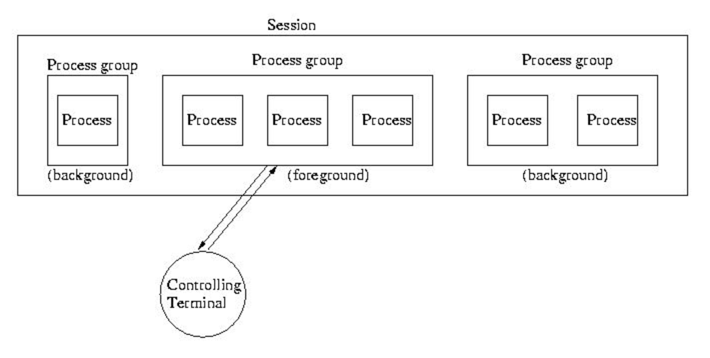
\includegraphics[width=200px, height=150px]{controlling_terminal.png}
        \caption{Schéma montrant un terminal de contrôle désigné pour un groupe de processus}
\end{figure}

Les \textit{jobs} sur Linux représentent des processus qui peuvent être de trois types principaux : \textit{avant-plan}, \textit{arrière-plan} et \textit{suspendu}. Lorsqu'un utilisateur exécute une commande dans le shell, un processus est créé pour exécuter cette commande. Si ce processus nécessite une interaction immédiate avec l'utilisateur, il est exécuté en \textit{avant-plan}, ce qui signifie que l'utilisateur doit attendre la fin de son exécution avant de pouvoir utiliser à nouveau le shell.

En revanche, si l'utilisateur souhaite libérer le shell pour d'autres commandes tout en laissant le processus s'exécuter en arrière-plan, il peut le démarrer en tant que \textit{job arrière-plan}. Cela permet à l'utilisateur de continuer à travailler dans le shell pendant que le processus s'exécute en tâche de fond.

Le type \textit{suspendu} se réfère à un \textit{job} qui a été temporairement stoppé, généralement par une combinaison de touches comme Ctrl-Z. Il peut ensuite être repris en arrière-plan ou en avant-plan.

\begin{tcolorbox}[title=Comment savoir quel est mon terminal de contrôle?]
Pour savoir quel terminal de contrôle est attaché au \textit{shell} en cours d'exécution, il suffit d'utiliser la commande : \textbf{tty}. Cette commande affichera le chemin absolu du terminal de contrôle qui \textit{contrôle} ce \textit{shell}. Si vous utilisez cette commande sur un émulateur de terminal, le terminal de contrôle sera le pseudo-terminal esclave rattaché au processus qui exécute le \textit{shell}. Dans le cas des consoles virtuelles (voir le chapitre concernant le terminal virtuel), il n'y a pas de notions de pseudo-terminaux. Le noyau simule un terminal physique directement et rattache ce terminal de contrôle à la console virtuelle.
\end{tcolorbox}

\begin{tcolorbox}[title=Utilisation de la commande sur l'émulateur de terminal]
\begin{verbatim}
user@localhost:~/Documents>tty
/dev/pts/2
user@localhost:~/Documents>_
\end{verbatim}
\end{tcolorbox}

\begin{tcolorbox}[title=Utilisation de la commande sur la console virtuelle]
\begin{verbatim}
user@localhost:~>
/dev/tty2
user@localhost:~>_
\end{verbatim}
\end{tcolorbox}

\section{Le programme pilote}
Avec tout ce bagage d'informations, nous connaissons plus ou moins les bases du fonctionnement des terminaux et pseudo-terminaux. Cependant, un problème subsiste : comment les entrées au clavier sont-elles interprétées par le maître ? \textit{Est-ce que c'est l'extrémité maître du pseudo-terminal qui récupère les entrées directement du clavier ?} La réponse est bien sûr que \textbf{non}.

Comme dit plus haut, l'émulateur de terminal est un processus qui tourne dans le système. Il possède son propre \textit{pid} et on peut même aller vérifier qui est son parent. Il n'y a pas de hasard sur Linux. Sachant que l'émulateur de terminal est directement rattaché à l'extrémité maître, c'est le seul processus qui peut être capable d'intercepter les données entrées sur le clavier.

Dans le livre de \textit{Michael Kerrisk} sur \textit{The Linux Programming Interface}, il fait référence à un programme pilote qui renvoie les entrées au clavier directement à l'extrémité maître, sans pour autant expliquer ce qu'est ce \textit{programme pilote}. Après plusieurs recherches, c'est le \textit{serveur d'affichage} sur Linux qui reçoit des \textit{events} de la part des pilotes (clavier, etc..). D'ailleurs une explication rapide avait été donné dans le chapitre \textit{Terminal virtuel} dans la section \textit{pilote de terminal}.

\hfill \break

Le serveur d'affichage (par exemple : X11) reçoit les \textit{events} et transmet l'information au programme qui tourne, dans notre cas, c'est l'émulateur de terminal. On s'aperçoit très vite que le \textit{programme pilote} dont Kerrisk parlait était en fait l'émulateur de terminal. Et ceci colle très bien, c'est bien l'émulateur de terminal qui envoie les données à l'extrémité maître et le maître renvoie les données en entrée à l'extrémité esclave.

\begin{figure}[h]
	\centering
	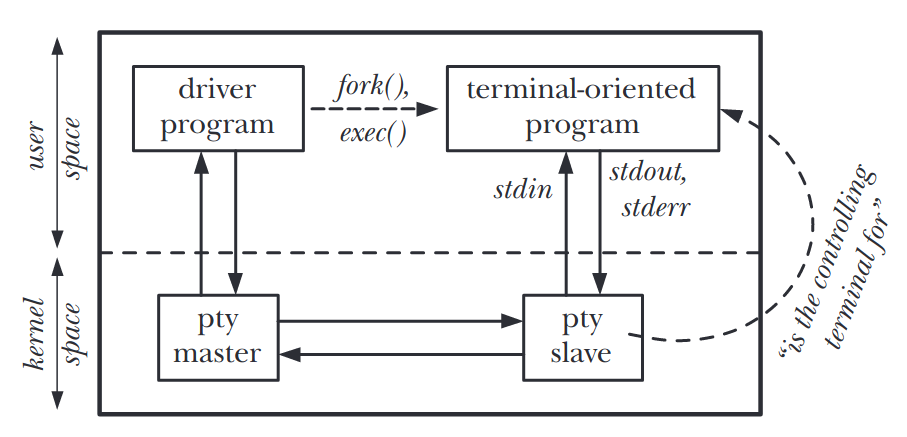
\includegraphics[width=200px, height=120px]{pseudo-terminal.png}
	\caption{Schéma montrant la communication entre 2 processus en utilisant le pseudo-terminal}
\end{figure}

Sur le schéma ci-dessus, les deux processus se distinguent : d'un côté, le \textit{programme pilote}, de l'autre, le \textit{bash}. On remarque l'inscription \textit{terminal-oriented program}, ce qui signifie simplement qu'il s'agit d'un programme ayant besoin de 'quelque chose' simulant un terminal. Et cette 'quelque chose' n'est autre que l'extrémité esclave, jouant le rôle de terminal de contrôle pour le programme. En quelque sorte, le programme 'pense' qu'il utilise un terminal.
